% Source: graduate-coursework/Research/Papers/drafts/temporal_context_motion_trails/Radar_TemporalContext_MotionTrails.tex
% Description: Clutter sensitivity increases with horizon as persistent trails generate spurious structure.

\documentclass[border=4pt]{standalone}
\usepackage{algpseudocode}
\usepackage{amsmath,amssymb}
\usepackage[T1]{fontenc}
\usepackage{pgfplots}
\usepackage{tikz}
\usepackage{xcolor}
\pgfplotsset{compat=1.18}
\usetikzlibrary{arrows.meta,positioning,calc,fit,shapes.geometric,shapes.misc,decorations.pathmorphing,backgrounds}


\newcommand{\ph}[1]{\textcolor{red}{#1}}

\begin{document}
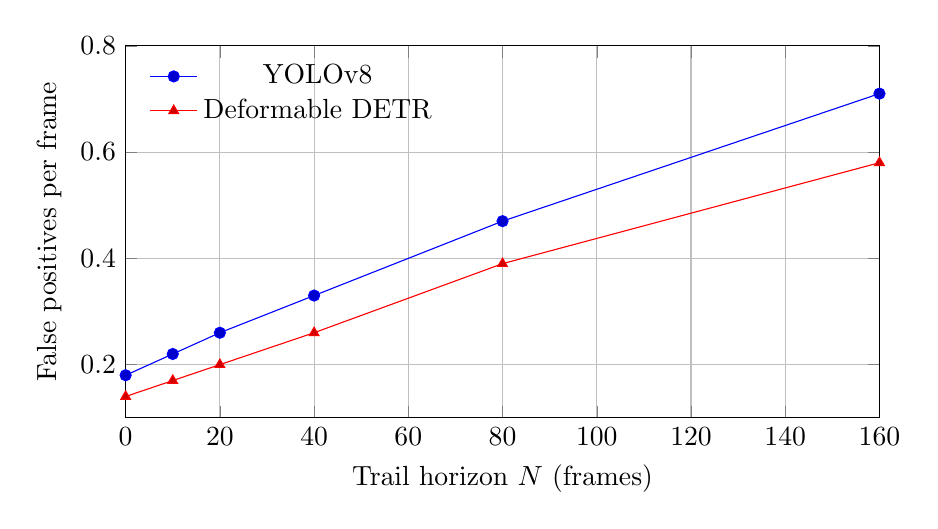
\begin{tikzpicture}
\begin{axis}[
  width=0.92\linewidth,
  height=0.52\linewidth,
  xlabel={Trail horizon $N$ (frames)},
  ylabel={False positives per frame},
  xmin=0, xmax=160,
  ymin=0.10, ymax=0.80,
  grid=both,
  legend style={at={(0.02,0.98)},anchor=north west,draw=none,fill=none},
]
\addplot+[mark=*] coordinates {(0,0.18) (10,0.22) (20,0.26) (40,0.33) (80,0.47) (160,0.71)};
\addlegendentry{YOLOv8}
\addplot+[mark=triangle*] coordinates {(0,0.14) (10,0.17) (20,0.20) (40,0.26) (80,0.39) (160,0.58)};
\addlegendentry{Deformable DETR}
\end{axis}
\end{tikzpicture}
\end{document}
